\documentclass[a4paper]{article}
\usepackage[spanish]{babel}
\usepackage[utf8]{inputenc}
\usepackage{charter}   % tipografia
\usepackage{graphicx}
%\usepackage{makeidx}
\usepackage{paralist} %itemize inline
\usepackage{enumitem}
\usepackage{color} % para snipets de codigo coloreados
\usepackage{fancybox}  % para el sbox de los snipets de codigo

\definecolor{litegrey}{gray}{0.94}

% \newenvironment{sidebar}{%
% 	\begin{Sbox}\begin{minipage}{.85\textwidth}}%
% 	{\end{minipage}\end{Sbox}%
% 		\begin{center}\setlength{\fboxsep}{6pt}%
% 		\shadowbox{\TheSbox}\end{center}}
% \newenvironment{warning}{%
% 	\begin{Sbox}\begin{minipage}{.85\textwidth}\sffamily\lite\small\RaggedRight}%
% 	{\end{minipage}\end{Sbox}%
% 		\begin{center}\setlength{\fboxsep}{6pt}%
% 		\colorbox{litegrey}{\TheSbox}\end{center}}

\newenvironment{codesnippet}{%
	\begin{Sbox}\begin{minipage}{\textwidth}\sffamily\small}%
	{\end{minipage}\end{Sbox}%
		\begin{center}%
		\vspace{-0.4cm}\colorbox{litegrey}{\TheSbox}\end{center}\vspace{0.3cm}}




\usepackage{fancyhdr}
\usepackage{natbib}
\pagestyle{fancy}

\renewcommand{\sectionmark}[1]{\markright{\thesection\ - #1}}

\fancyhf{}

\fancyhead[LO]{Sección \rightmark} % \thesection\ 
\fancyfoot[LO]{\small{Leandro Raffo, Maximiliano Fernández Wortman, Uriel Rozenberg.}}
\fancyfoot[RO]{\thepage}

\renewcommand{\headrulewidth}{0.5pt}
\renewcommand{\footrulewidth}{0.5pt}
\setlength{\hoffset}{-1.1in}
\setlength{\textwidth}{18cm}
%\setlength{\hoffset}{-1.1cm}
%\setlength{\textwidth}{16cm}
\setlength{\headsep}{0.5cm}
\setlength{\textheight}{25cm}
\setlength{\voffset}{-0.7in}
\setlength{\headwidth}{\textwidth}
\setlength{\headheight}{13.1pt}

\renewcommand{\baselinestretch}{1.1}  % line spacing


%\usepackage{etoolbox}
%\patchcmd{\bibliography}{\section*}{\section}{}{}

% \setcounter{secnumdepth}{2}

\usepackage{caratula}


\begin{document}


\thispagestyle{empty}
\materia{Organización del Computador II}
\submateria{Segundo Cuatrimestre de 2015}
\titulo{Trabajo Práctico II}
\subtitulo{Programacion SIMD}
\integrante{Leandro Raffo}{}{}
\integrante{Maximiliano Fernández Wortman}{}{}
\integrante{Uriel Rozenberg}{}{}

%Pagina de titulo e indice
%\thispagestyle{empty}

\maketitle 

\tableofcontents

\newpage

\section{Introduccion}
En este trabajo práctico realizamos la implementación de dos filtros de imagenes, con tal de ver que tan eficiente puede llegar a ser (o no) SIMD, los filtros son la diferencia de imagenes y el blur gaussiano, los cuales fueron implementados en lenguaje C (gcc y clang) y assembly, haciendo uso de instrucciones vectoriales. Luego comparamos la performance de estas implementaciones sobre diferentes imagenes y usando herramientas probabilísticas y estadísticas.

\section{Implementacion}

\subsection{Diferencia}
 Descripcíon de un ciclo de la iteración del filtro diferencia.\\
Primermo pedimos memoria para declarar las máscaras que vamos a usar y armamos el stackframe (omitido)
\begin{codesnippet}
\begin{verbatim}
section .rodata
mascara_copia_pixels db 2,2,2,2,6,6,6,6,10,10,10,10,14,14,14,14
mascara_asigna_alpha db 0,0,0,255,0,0,0,255,0,0,0,255,0,0,0,255
\end{verbatim}
\end{codesnippet}

 Luego de armar el stackframe tenemos
\begin{codesnippet}
\begin{verbatim}
mov r12, rdx
mov eax, r8d
mov ecx, ecx
mul rcx
xor r15, r15
\end{verbatim}
\end{codesnippet}
r12 apunta a la matriz resultado, ecx tiene la cantidad de filas, y la parte baja de rax(eax) tiene la cantidad de columnas. Al hacer mul rcx se tiene filas*columnas en rdx:rax, como movimos cosas de 32 bits obtenemos la multiplicación en rax, que es lo que vamos a usar, junto a r15 para iterar (notar que tenemos en cuenta para esto que los movimientos de registros entre dwords limpian la parte alta de los registros de 64bits, es decir extendemos el número usando que son enteros positivos). Ahora entramos al ciclo.

\begin{codesnippet}
\begin{verbatim}
.ciclo:
    cmp r15, rax
    JE .fin
\end{verbatim}
\end{codesnippet}

 Comparamos si r15 es igual a rax en tal caso ya hicimos la diferencia sobre todos los pixeles y termina el ciclo. El ciclo sigue con

\begin{codesnippet}
\begin{verbatim}
    movdqu xmm3 , [RDI +  r15*4]   
    movdqu xmm15, [RSI +  r15*4]
    movdqu xmm14, xmm15     
    pminub xmm15, xmm3        
    pmaxub xmm3 , xmm14        
    psubb  xmm3 , xmm15             
    movdqu xmm4, xmm3 
    movdqu xmm5, xmm3       
\end{verbatim}
\end{codesnippet}

 Movemos a xmm$3$ los primeros $4$ pixeles de la primera matriz y a xmm$15$ los primeros $4$ de la segunda matriz a comparar, estos ocupan respectivamente $16$ bytes en memoria (brga por $4$). Después Guardamos en xmm$14$ el valor de xmm$15$ y hacemos un pminub entre xmm$15$ y xmm$3$ lo cual deja en xmm$15$ el mínimo byte a byte. Lo mismo para xmm$3$ pero con pmaxub es decir este tiene el máximo byte a byte. Hacemos esto porque queremos calcular el valor absoluto de la forma $|x-y|$ = $\max(x,y) - \min(x,y)$. Concluimos esta idea haciendo psubb entre xmm$3$ que tenia el máximo y xmm$15$ que tenia el mínimo y finalmente guardamos el resultado en xmm$4,5$ para operar en la siguiente parte.

\begin{codesnippet}
\begin{verbatim}
    pslldq xmm4, 1                  
    pslldq xmm5, 2               
    movdqu xmm6, xmm5             
    pmaxub xmm6, xmm4             
    pmaxub xmm6, xmm3              
    pshufb xmm6, [mascara_copia_pixels] 
    paddsb xmm6, [mascara_asigna_alpha]
    movdqu [r12 +  r15*4], xmm6
    add  r15d, 4
    jmp .ciclo
\end{verbatim}
\end{codesnippet}

 Ahora shifteamos con packed shift xmm$4,5$ uno y dos bytes respectivamente de forma de poder tomar el máximo de entre r g b en paralelo, es decir $4$ pixels a la vez. Por ejemplo, el primer byte de xmm$4$ tiene al byte de r, y el de xmm$6$ tiene al byte de g, de forma que al hacer pmaxub entre  xmm$6$ y xmm$4$ nos deja en el primer byte de xmm$6$ (y cada 3 bytes) max(r$_n$,g$_n$) donde $n = \{1,2,3,4 \}$ indican los pixeles que levantamos. Los demas bytes de este registro no nos interesan. Repetimos esto entre xmm$6$ y xmm$3$, pasa de vuelta lo mismo pero ahora tenemos en el primer byte de xmm$6$ (y cada $3$ bytes) max(r$_n$,g$_n$,b$_n$) con $n = \{1,2,3,4 \}$. Ahora tenemos que mover este máximo a las 3 coordenadas r, g y b, hacemos esto mediante la mascara mask$_5$ y mediante trans$_2$ sumamos con saturación con tal de dejar en alpha el valor $255$. Copiamos los 16 bytes correspondientes (con el offset adecuado) en la matriz destino, sumamos $4$ a r$15$d y saltamos para, si es necesario, volver a hacer el ciclo completo.


\subsection{Blur gaussiano}

 El blur gaussiano consta de dos ciclos uno anidado sobre el otro, el anidado itera sobre el kernel y el que anida itera sobre la matriz, usamos SIMD para hacer los calculos sobre cuatro pixeles en simultaneo (es decir sobre 16 componentes en total), además en vez de hacer offsets para atras como el codigo en C nos movemos siempre para adelante, por ejemplo, empezamos en el pixel $0$ y recorremos la submatriz que va de $0, 2r$ en filas y $0, 2r$ en columnas, donde $r$ es el radio, a la par de la matriz del kernel (que también tiene este tamaño) haciendo las multiplicaciones sobre cuatro pixeles y acumulandolas, luego cuando terminamos de iterar sobre el kernel, insertamos en los cuatro pixel destino, que esta en la posición ($r, r$) hasta ($r+3, r+3$), luego aumentamos la columna y seguimos este proceso hasta el ancho $- 2r - 16$ donde nos paramos en la proxima fila y repetimos hasta llegar a la altura $- 2r$, es decir siempre que insertamos los pixeles estamos en rango. Podemos hacer 4 pixeles a la vez pues el ancho es un múltiplo de 4. Ahora pasamos a describir más en detalle las operaciones que usamos para esto. \newline
 
\noindent \textbf{Nota:} Siempre vamos a poner el código sobre un pixel porque las operaciones sobre los otros 3 son las mismas operaciones sobre distintos registros en seguidilla, vamos a aclarar estos casos en la explicación.
\newline

 Antes de entrar al ciclo preparamos algunos registros para saber hasta donde iterar, tenemos que: rax guarda el último valor hasta el que vamos a recorrer que es igual a  [(filas $- 2r$)*columnas] $-2r$, rbp va a guardar hasta donde vamos a hacer cada subciclo es decir $(2r+1)^2$, r11 tiene el valor $2r$, r12 la matriz fuente, r13 la matriz destino, r8 la cantidad de columnas y rbx (ebx) el offset necesario para insertar el pixel en la matriz destino.
\begin{codesnippet}
\begin{verbatim}
.ciclo_kernel:
    cmp rcx, rbp                      
    je .insert          
    mov r9, rsi
    add r9, rdi
    movd        xmm0, [ r12 + r9 ]      
    punpcklbw   xmm0, xmm8              
    punpcklwd   xmm0, xmm8              
    cvtdq2ps    xmm0, xmm0    
\end{verbatim}
\end{codesnippet}

 Primero verificamos si tenemos que insertar el pixel, para esto comparamos rcx, el registro que cuenta sobre el tamaño del kernel contra rbp que mantenia hasta donde teniamos que iterar para haber recorrido el kernel, si no, levantamos de memoria 4 bytes y los desempaquetamos a double words y convertimos a float, repetimos esto con los offsets $r12 + r9 + 4/8/12$, es decir los primeros $16$ bytes, y guardando en los registros xmm4, xmm5 y xmm6 respectivamente.
\begin{codesnippet}
\begin{verbatim}    
    movd        xmm1, [ r10 + rcx*4 ]   
    movq        xmm3, xmm1              
    pslldq      xmm3, 4
    paddd       xmm3, xmm1              
    pslldq      xmm3, 4
    paddd       xmm3, xmm1                           
    mulps       xmm0, xmm3              
    addps       xmm2, xmm0              

\end{verbatim}
\end{codesnippet}

Como rcx itera el kernel linealmente, movemos el valor de la matriz de convolución apuntado por rcx con movd (un float por eso el *$4$) a xmm1, shifteamos 4 bytes con pslldq, ya que queremos propagar este valor para que multiplique las 3 componentes (rgb) a la vez, movemos un quadword shifteamos y hacemos un packed add (queremos copiar el valor del float) shifteamos xmm3 y volvemos a sumar una vez más, para que cada doubleword de xmm3 tenga el flaot. Luego multiplicamos el registro con el valor del pixel del kernel, contra los valores del pixel que desempaquetamos en xmm0 dejando en xmm0 este valor y lo acumulamos en xmm2. De vuelta repetimos esto con $xmm4/5/6$ y acumulamos en $xmm7/9/10$

\begin{codesnippet}
\begin{verbatim}
    cmp rdx, r11
    je .sumar_fila_kernel
    add rdx, pixel_size
    inc rcx
    add rsi, pixel_size
    jmp .ciclo_kernel
\end{verbatim}
\end{codesnippet}

rdx mantiene el contador para iterar sobre la fila, si este es igual a 2r saltamos a sumar\_fila\_kernel de lo contrario adelantamos rdx y rsi en pixel\_size (que es un \%define con el valor $4$) y entramos al ciclo de vuelta.


\begin{codesnippet}
\begin{verbatim}
.sumar_fila_kernel:
    xor rdx, rdx
    sub rsi, r11                      
    add rsi, r8                        
    inc rcx
    jmp .ciclo_kernel
\end{verbatim}
\end{codesnippet}


 En sumar fila limpiamos rdx, para volver a poder iterar de $0$ a $2r$, le restamos $2r$ a rsi, este iteraba sobre la fila para la matriz mas grande y le sumamos al mismo la cantidad de columnas, es decir rsi apunta al comienzo de la fila siguiente, incrementamos rcx asi en el proximo ciclo apunta a la siguiente fila tambien y saltamos al ciclo de vuelta.

\begin{codesnippet}
\begin{verbatim}
 .insert:
    pxor     xmm4, xmm4
    cvtps2dq xmm2, xmm2                 
    packusdw xmm2, xmm4                 
    packuswb xmm2, xmm4                 
    movd     xmm7, ebx
    add      rbx, rdi
    movd     [ r13 + rbx ], xmm2           
    ..
    movd	 [ r13 + rbx + 4], xmm7
    ..
    movd     ebx, xmm7
    pxor     xmm7, xmm7
    xor rsi, rsi
    xor rcx, rcx
    cmp rdi, r15
    je .sumar_fila
    add rdi, pixel_size
    jmp .ciclo_matriz
\end{verbatim}
\end{codesnippet}

En .insert hacemos casi lo contrario a levantar, convertimos los floats empaquetados que estaban en xmm2 a doublewords empaquetados y re-empaquetamos a word y luego a byte. Luego sumamos rbx e rdi para obtener la posición en la que vamos a insertar el pixel (los 4 bytes) e insertamos el pixel, de vuelta repitiendo para los 4 pixeles con el offset $+4/8/12$. Una vez que esto pasa ponemos rsi y rcx en $0$ y vemos si llegamos a la ultima columna que teniamos que iterar, si pasa esto saltamos a sumar\_fila sino sumamos 4*pixel\_size a rdi y saltamos al ciclo del kernel de vuelta.

\begin{codesnippet}
\begin{verbatim}
.sumar_fila:
    add rdi, r11                 
    add r15, r8                    
    jmp .ciclo_matriz
\end{verbatim}
\end{codesnippet}

 En .sumar\_fila lo que hacemos es sumarle a rdi lo que faltaba para llegar a la proxima columna, $2r$ y le sumamos a r15 la cantida de columnas, r15 en este caso mantiene (acorde al rdi) hasta que columna tenemos que iterar. Basicamente r15 empieza en cols $-2r$ y se le van sumando el total de columnas, en la segunda iteracion tiene $2$cols $-2r$ etc. Aca saltamos a ciclo\_matriz y no ciclo\_kernel, este contiene lo siguiente.

\begin{codesnippet}
\begin{verbatim}
.ciclo_matriz:
    cmp rdi, rax                       
    jg .end
\end{verbatim}
\end{codesnippet}

 Si rdi es mayor que rax (que marcaba el ultimo pixel sobre el que podiamos iterar) saltamos al final, desarmamos el stackframe y retornamos.

\section{Resultados}

\subsection{Diferencia}

\noindent \textbf{Nota:} todos los tests fueron corridos sobre una PC con procesador Intel Core2Duo E8400 que cuenta con 64kb de cache L1 para datos, 64kb de cahce L1 para instruccionnes y 6mb de cache L2 compartido para data e instrucciones por los dos nucleos.
\\
\newline
 Para analizar las implementaciones de C y assembly, corrimos 1000 iteraciones de cada implementación de diferencia sobre una imagen de 2308x2308 (16mb) donde las implementaciones de C se compilaron con gcc y clang usando los flags de optimización -O0, -O1, -O2, -O3 y -Os. Basicamente los flags de -O\# con \# un número entre $0,3$ intentan optimizar principalmente para velocidad y luego tamaño, $0$ siendo el menos 'optimizado' y $3$ el más optimizado, mientras que -Os optimiza principalmente por tamaño del ejecutable, por ejemplo, luego de hacer un disassembly, notamos que a partir de -O2 gcc ya no armaba un stackframe, ni resguardaba rbp, y pusheaba a medida que necesitaba los registros, alineando rsp cuando fuese necesario usar la pila, diferencias observables entre -O2 y -O3 fue el uso de operaciones SIMD, por ejemplo de empaquetado y desempaquetado, multiplicaciones packed etc en -O3 (para el blur), mientras que esto no pasaba en -O2, extrañamente la performance es la misma y tal vez se debe a otros factores como el modelo de procesador (Intel c2d E840) o que en general gcc hace muchos mas accesos a memoria y estos hacen sombra a la performance ganada por las instrucciones. \newline


 A continuación dejamos los gráfico con el promedio (con y sin outliers) de la diferencia bajo distintos flags de optimización y en assembly.

 
%REHACER 
\begin{figure}[h]
\centerline{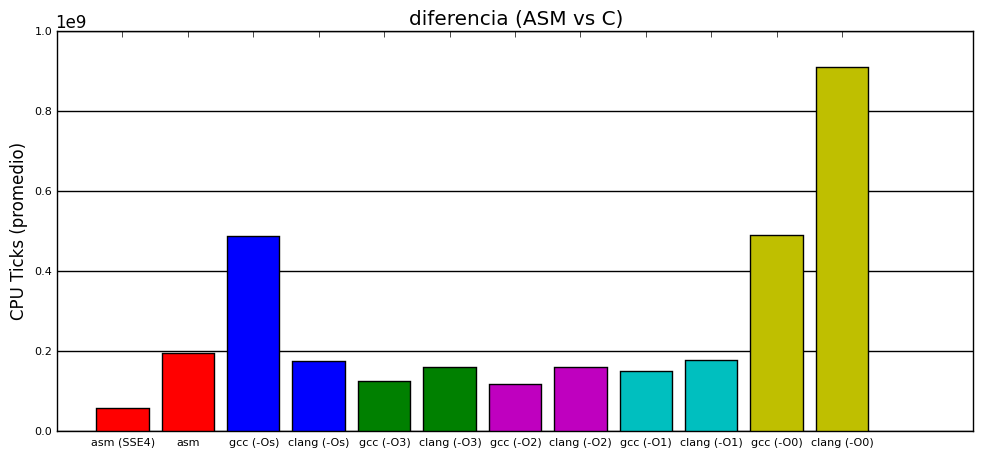
\includegraphics[scale=0.71]{imagenes/test_difrencia_ASM_C_PROMEDIO_Os}}
\caption{Promedio, 1000 iteraciones sobre una imagen de 2308x2308 pixels de 16mb.}
\end{figure}

Como podemos observar, la versión en assembler usando instrucciones vectorizadas es más de dos veces mas rapida que cualquiera de las otras implementaciones. En particular es. Otra cosa a observar es que la versión en assembler usando registros de propósito general es más lenta que cualquiera de las versiones -O3 y -O2 de los compiladores, leyendo el manual de optimización de intel vimos en la sección 3.5.1.5 y citamos: "Avoid ROTATE by register or ROTATE by immediate instructions. If possible, replace with a ROTATE by 1 instruction."
Interesantemente al reemplazar los ror rax, 8 por ror rax, 1 y desplegar en 8 instrucciones (4 veces se hacia cada ror por lo tanto 24 instrucciones) vimos drásticamente afectada la performance del algoritmo, pero para mal, es decir corre más lento que cualquiera de las otras implementaciones. Dejamos a continuación los valores númericos del promedio la desviación, la mediana y la esperanza.


\begin{center}
        \begin{tabular}[c]{|c|c|c|c|c|}
    \hline
        \textbf{Tipo} &  \textbf{Esperanza} & \textbf{Desviación} & \textbf{Mediana}\\
        \hline
\textit{asm (SSE)} &  56.043.648  & 3.719.499 & 54.745.299\\
        \hline
\textit{asm} &   185.730.157    & 35.225.868 & 163.627.996 \\
		\hline
\textit{gcc -Os} &  483.066.761   & 86.386.164 & 425.219.445\\
        \hline
\textit{gcc -O3} &  122.860.749 & 23.118.334 & 106.125.907\\
        \hline
\textit{gcc -O2} &  116.990.809 & 22.296.448 & 100.375.353\\
        \hline
\textit{gcc -O1} & 152.638.557 & 28.306.860 & 133.249.693\\
        \hline
\textit{gcc -O0} & 484.505.949  & 84.107.766 & 441.267.745\\
        \hline
\textit{clang -Os} &  175.719.296 & 32.586.563 & 153.610.569\\
        \hline
\textit{clang -O3} &   162.637.196 & 31.045.244 & 139.688.334\\
        \hline
\textit{clang -O2} &    159.943.847 & 29.501.029 & 139.728.946\\
        \hline
\textit{clang -O1} &    178.052.400  & 33.145.132 & 155.390.607\\
        \hline
\textit{clang -O0} & 932.036.522  & 148.813.063 & 896.191.006 \\
        \hline
    \end{tabular}
\end{center}

%REHACER

Además de esto escribimos varias versiones de assembler usando registro de propósito general, a las cuales llamaremos asm v1-4. Ahora pasamos a explicar brevemente como estan implementadas.

\begin{itemize}[label={}]
\item[] \textbf{asm v1:} Levanta de a 8 bytes y luego trabaja sobre estos 2 pixeles por medio de shifts rotaciones y dos llamadas a una funcion que calcula la norma infinito de los mismos.
\item[] \textbf{asm v2:} Lo mismo que lo anterior, excepto que las rotaciones por inmediatos estan 'desenrolladas' por varias llamadas a ror reg, 1, esto viene de que al leer el manual de optimización de intel nos encontramos con y cito: section 3.5.1.5: ``avoid ROTATE by register or ROTATE by immediate instructions. If possible, replace with a ROTATE by 1 instruction."
\item[] \textbf{asm v3:} Una idea parecida a v1, excepto que en vez de rotaciones usamos puramente shifts.
\item[] \textbf{asm v4:} Lo mismo que v3 pero las llamadas a la función que calcula las normas infinitos estan inlineadas
\item[] \textbf{asm v5:} Lo mismo que v4, solo que ahora la función que aplica la norma infinito tiene menos instrucciones y opera sobre 4 bytes en vez de 8 por ciclo.
\end{itemize}

En general se intento evitar accesos a memoria, comparado a lo que hace gcc que son 15+ accesos por iteración, hacemos 3 accesos a memoria pidiendo entre 8 a 4 bytes.

Pasamos todas estas implementaciones sobre 2000 iteraciones sobre una imagen de 16mb de 2308x2308 pixels y obtuvimos los siguientes resultados:

\begin{figure}[h]
	\centerline{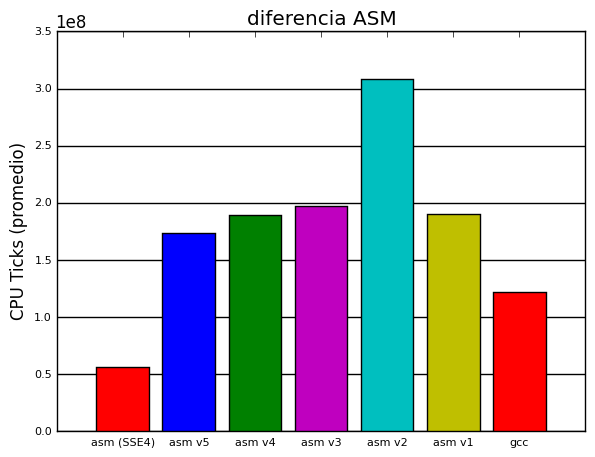
\includegraphics[scale=1]{imagenes/test_diferencia_ASM_imp}}
	%\caption{Diferencia en asm, escala logarítmica}
\end{figure}

\begin{center}
        \begin{tabular}[c]{|c|c|c|c|c|}
    \hline
        \textbf{Tipo} &  \textbf{Esperanza (ticks)} & \textbf{Desviación (ticks)} & \textbf{Mediana (ticks)}\\
        \hline
\textit{asm (SSE)} &    56.680.048  & 2.023.564 & 56.059.389\\
        \hline
\textit{asm v5} &   173.458.584    & 33.815.428 & 149.441.206\\
        \hline
\textit{asm v4} &   189.075.813    & 37.004.652 & 162.500.233 \\
        \hline
\textit{asm v3} &  197.540.668  & 38.514.532 & 169.892.176\\
        \hline
\textit{asm v2} &  307.955.171   & 59.536.896 & 262.879.128\\
        \hline
\textit{asm v1} &  189.969.936 & 37.223.783 & 162.727.425\\
        \hline
\textit{gcc -O3} &  121.772.855 & 23.099.911 & 105.157.858\\
        \hline
    \end{tabular}
\end{center}

Como se puede apreciar, la Esperanza (media aritmética sobre el total de iteraciones) de la versión SSE es \textbf{2.14} veces más rápida que la version de gcc con flag de optimización -O3, además su desviación es mucho más pequeña que cualquiera de las otras implementaciones, lo cual muestra que es mucho más estable, esto pasa en general para la mayoria de las implementaciones que hicimos en assembler.

Por otro lado ninguna de las versiones que usan solo registros de propósito general pasan en velocidad a la versión de gcc, creemos que esto se debe a que gcc esta alineando su código por medio de operaciones nops para que tenga mejor branching.



Una de nuestras hipótesis era que el tamaño del cache iba a afectar la performance de nuestro algoritmo. Para esto corrimos la diferencia en Assembly y C sobre imágenes que iban de 64kb a 64mb como se ve en la figura, de vuelta bajo gcc y clang, pero esta vez con el flag de optimización -O2, ya que por el test anterior era el que mejor se comportaba sobre la diferencia. 

\begin{figure}[h]
	\centerline{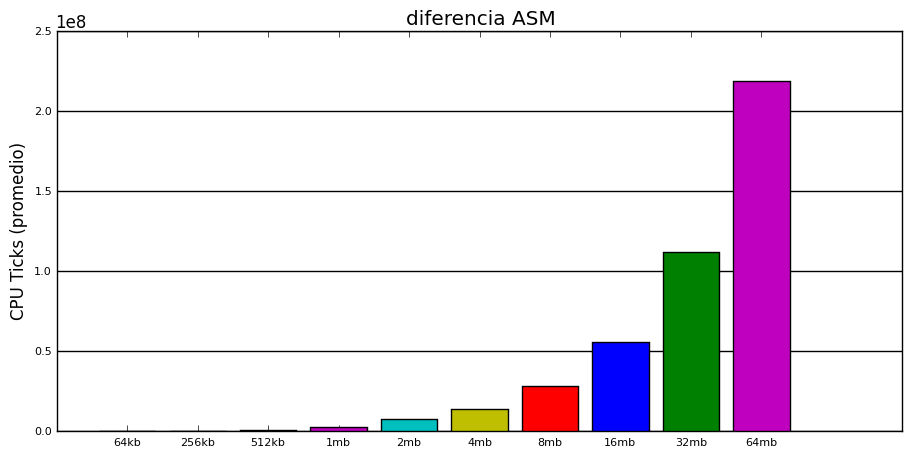
\includegraphics[scale=0.78]{imagenes/test_performance_size_ASM_bar.png}}
	\caption{Diferencia en asm, escala logarítmica}
\end{figure}

Y los siguientes valores


\begin{center}
        \begin{tabular}[c]{|c|c|c|c|c|}
    \hline
        \textbf{Tipo} &  \textbf{Esperanza (ticks)} & \textbf{Desviación (ticks)} & \textbf{Mediana (ticks)}\\
        \hline
\textit{64kb} &    78.063  & 223.209 & 60.300\\
        \hline
\textit{256kb} &   368.823    & 286.970 & 291.676\\
        \hline
\textit{512kb} &  1.017.418   & 960.937 & 860.229 \\
        \hline
\textit{1mb} &  2.923.201  & 1.160.558 & 2.530.638\\
        \hline
\textit{2mb} &  7.912.487   & 1.085.181 & 7.547.283\\
        \hline
\textit{4mb} &  14.056.689 & 1.302.569 & 13.741.051\\
        \hline
\textit{8mb} &  28.452.651 & 1.293.358 & 28.296.252\\
        \hline
\textit{16mb} &  55.610.396 & 2.150.184 & 55.004.058\\
        \hline
\textit{32mb} &  112.007.095 & 2.896.770 & 111.689.064\\
        \hline
\textit{64mb} &  219.320.476 & 2.945.521 & 218.553.592\\
        \hline
    \end{tabular}
\end{center}

Recordemos brevemente que nuestro procesador tiene dos niveles de cache, un primer L1 con 64kb para datos y otros 64kb para instrucciones y un segundo nivel L2 compartido por ambos y además compartido por los dos cores. Mirando la tabla vemos que una vez que tenemos una imagen mas grande que el L1D, tenemos un incremento de 4.7 veces más ciclos en vez de 4, que es lo que se esperaria al cuadruplicar el tamaño de la imagen. Luego tenemos otro crecimiento mayor de 1mb a 2mb, donde en vez de tardar el doble tarda 2.7 veces más, una vez que pasamos la barrera de los 6mb, nuestro algoritmo sigue creciendo pero parece que tiende a $2$ ciclos\_medida\_anterior, que es lo que esperariamos de doblar el tamaño de las imágenes.
Luego de hacer esto corrimos cachegrind, que es una herramienta que viene con el programa Valgrind que sirve para analizar el cache y los branches, en un par de casos particulares para observar que está pasando con la cache. Notemos que LL es last level cache que en este caso para el Core2Duo es el nivel L2.
\begin{center}
	\begin{tabular}[c]{|c|c|c|c|c|c|c|}
    \hline
        \textbf{asm} &  \textbf{L1i miss rate} & \textbf{LLi miss rate} & \textbf{L1d miss rate} & \textbf{LLd miss rate} & \textbf{LL miss rate} & \textbf{branch mispredict}\\
        \hline
\textit{64kb} &    0.01\%  & 0.01\% & 12.9\% & 0.2\% & 0.0\% & 0.9\% \\
        \hline
\textit{256kb} &   0.00\%    & 0.00\% & 13.1\% & 0.1\% & 0.0\% & 0.2\% \\
        \hline
\textit{512kb} & 0.00\%    & 0.00\% & 13.1\%   &   0.1\% & 0.0\% & 0.01\% \\
        \hline
\textit{1mb} &  0.00\%    & 0.00\% & 13.1\%  & 0.00\%  & 0.0\% & 0.00\% \\
        \hline
\textit{2mb} &  0.00\%    & 0.00\% & 13.1\% & 13.0\% & 2.7\% & 0.00\% \\
        \hline
\textit{8mb} &  0.00\%    & 0.00\% & 13.1\% & 13.1\% & 2.7\% & 0.00\% \\
        \hline
    \end{tabular}
    
    
    	\begin{tabular}[c]{|c|c|c|c|c|c|c|}
    \hline
        \textbf{C} &  \textbf{L1i miss rate} & \textbf{LLi miss rate} & \textbf{L1d miss rate} & \textbf{LLd miss rate} & \textbf{LL miss rate} & \textbf{branch mispredict}\\
        \hline
\textit{64kb} &    0.01\%  & 0.01\% & 1.8\% & 0.2\% & 0.0\% & 0.9\% \\
        \hline
\textit{256kb} &   0.00\%    & 0.00\% & 1.8\% & 0.1\% & 0.0\% & 0.3\% \\
        \hline
\textit{512kb} & 0.00\%    & 0.00\% & 1.8\%   &   0.1\% & 0.0\% & 0.02\% \\
        \hline
\textit{1mb} &  0.00\%    & 0.00\% & 1.8\%  & 0.00\%  & 0.0\% & 0.01\% \\
        \hline
\textit{2mb} &  0.00\%    & 0.00\% & 1.8\% & 1.8\% & 0.3\% & 0.01\% \\
        \hline
\textit{8mb} &  0.00\%    & 0.00\% & 1.8\% & 1.8\% & 0.3\% & 0.00\% \\
        \hline
    \end{tabular}
\end{center}

Aca vemos varias cosas, por un lado, algo que era de esperarse es que el instruction miss rate sea bajísimo ya que nuestro binario esta siempre por debajo de 70kb. Por otro lado es notable ver que los miss rates de L1d se mantienen siempre por el 13\% contra los de gcc que están estables en 1.8\%, sin embargo nuestro algoritmo corre varias veces más rapido! El branch misprediction también era de esperarse que fuese bajo ya que iteramos casi linealmente sobre la matriz y no paramos hasta el final, los valores mas altos sobre las imagenes más pequeñas se lo adjudicamos a que el número de branches es mucho menor. De echo los mispredicts en assembler siempre rondan acerca de 5.000, mientras que gcc llega a alcanzar, en el último caso los 200.000, pero estos se ahogan sobre el total de branches que es todavía mucho mayor que la versión de assembler.

\newpage

\subsection{Blur}
Primero corrimos un tests parecido al de diferencia donde probamos todas las implementaciones de blur bajo distintos compiladores y tambien corrimos una versión vectorizada pero que solo trataba un pixel a la vez (sus 4 componentes) esta es llamada v1 y la que operaba 4 pixels (16 bytes) es llamada v2. Todo esto sobre una imagen de 1160x1160, radio $= 15$ y 100 iteraciones.

\begin{figure}[h]
	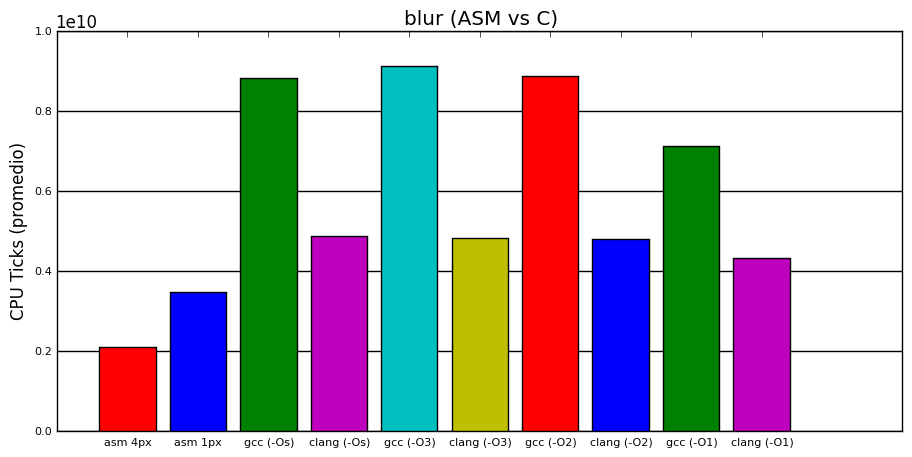
\includegraphics[scale=0.75]{imagenes/test_blur_ASM_C_.png}
	\caption{Promedio sobre 300 iteraciones del blur aplicado a una imagen de 1160x1160 con radio 3.}
\end{figure}

Como vemos la versión de assembler que opera sobre 4 pixels es más de 3 veces mas rápida que cualquiera de las versiones de C, y 1.6 veces más rapida que la versión que opera sobre un pixel, el cambio de codigo es entre un pixel y cuatro es mínimo, solo se usan mas registros pero se hacen las mismas operaciones y se cambia un offset, asi que no se justificaria nunca el no pasar a operar sobre 4 pixeles.


\begin{center}

        \begin{tabular}[c]{|c|c|c|c|c|}
    \hline
        \textbf{Tipo}  & \textbf{Esperanza} & \textbf{Desviación} & \textbf{Mediana}\\
        \hline
\textit{asm 4px} &	2.106.291.807 & 301.117.707 & 2.168.926.731 \\
		\hline
\textit{asm 1px} &	3.497.413.560 & 574.758.539 & 3.883.153.464 \\
		\hline
\textit{gcc -Os} &	8.843.585.499 & 1.578.879.058 & 10.084.543.303  \\
		\hline
\textit{gcc -O3} &	9.130.861.305 & 1.539.043.241 & 10.196.606.596  \\
		\hline
\textit{gcc -O2} &	8.896.692.812 & 1.594.654.086 & 10.158.618.532  \\
		\hline
\textit{gcc -O1} &	7.147.828.723 & 1.206.676.801 & 7.982.797.657  \\
		\hline
\textit{clang -Os} & 4.880.678.639 & 778.651.350 & 5.377.046.157  \\
		\hline
\textit{clang -O3} &	4.832.604.511 & 788.668.977 & 5.378.602.122  \\
		\hline
\textit{clang -O2} &	4.800.626.481 & 791.235.023 & 5.378.756.337  \\
		\hline
\textit{clang -O1} &	4.333.126.690 & 711.630.020 & 4.833.148.446  \\
		\hline
	\end{tabular}
\end{center}

 Otra cosa a notar es que el rol entre gcc y clang cambió, a diferencia de la diferencia de imagenes donde gcc era siempre mas rápido que clang aca pasa lo contrario, e inclusive la versión de clang en -O1 es la más rápida en general, esto también nos hace pensar que los flags de optimización no siempre son una solución efectiva si lo que se busca es codigo de alta performance. Una de las razones que creemos que c se comporta tan mal con el blur es por los saltos de fila, lo cual nos inclina a decir que ocurren muchos cache misses durante la iteración sobre el kernel, y esto no es la única perdida de performance, sino que además que gcc y clang utilizan el stack para guardar contadores y hacen varias multiplicaciones adentro del ciclo para calcular los offsets dentro de la matriz, lo cual nosotros pudimos evitar totalmente en la versión de assembler. 


 Otra de las hipótesis que teniamos con blur es que dada una imagen con un radio pequeño iba a correr mas lento que con un radio mas grande, pero a medida que el radio domine la cantidad de pixeles sobre las cuales va a aplicar la matriz de convolución el tiempo de ejecución iba a bajar. Esto lo pudimos probar corriendo blur sobre una imagen de tamaño fijo (en este caso 584x584 pixels) e incrementando el radio como se ve en la siguiente imagen


\begin{figure}[h]
	\centerline{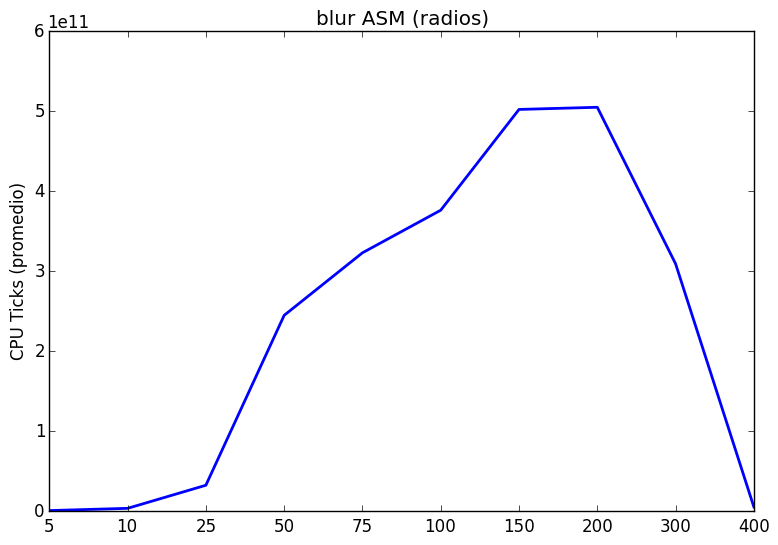
\includegraphics[scale=0.62]{imagenes/test_radio_size_ASM.png}}
	\caption{Blur, cambiando los radios}
\end{figure}


El algoritmo llega a un punto crítico cuando el radio es equivalente a la dimensión/2, es decir cuando el algoritmo se comporta como $O(n^4)$ sobre la dimensión, esto es fácil ver ya que dada una matriz cuadrada de tamaño $n^2$, si $r \sim n/2$, tenemos que por pixel hace $\sim n^2/2$ operaciones y hay $\sim n^2/2$ pixeles posibles para recorrer.

Al igual que en diferencia también corrimos, esta vez solo la versión assembler de blur sobre imágenes de tamaño 64kb a 32mb, radio 3 y sigma 1, obtuvimos lo siguiente:

\begin{figure}[h]
	\centerline{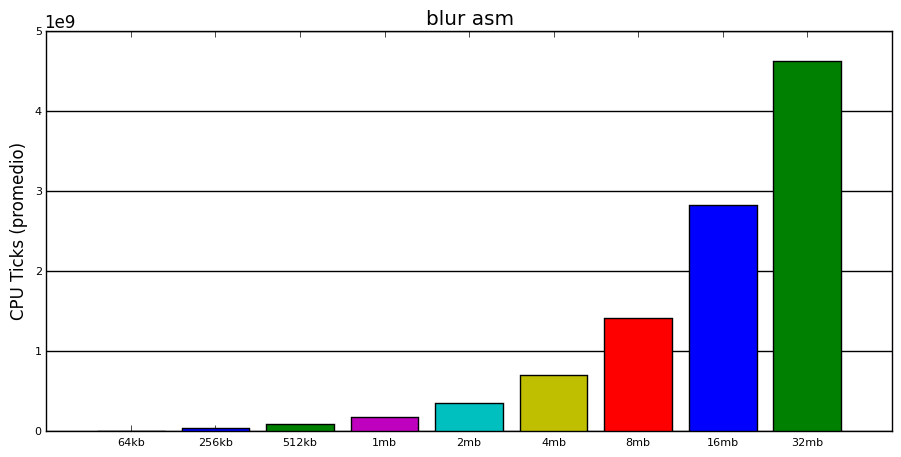
\includegraphics[scale=0.72]{imagenes/test_radio_cambiando_tamanios_assembly.png}}
	\caption{Blur, cambiando los radios}
\end{figure}

\newpage
\begin{center}
          \textbf{Test sobre tamaño}  \\ 
          \hfill \\
        \begin{tabular}[c]{|c|c|c|c|c|}
        \hline
      \textbf{Tipo}  & \textbf{Esperanza} & \textbf{Desviación} & \textbf{Mediana}\\
          	\hline
\textit{64kb} &	9.721.155 & 2.912.904 & 7.939.300 \\
		\hline

\textit{256kb} &	45.259.012 & 9.919.790 & 39.031.906 \\
		\hline
\textit{512kb} &	88.726.855 & 17.742.991 & 76.158.607 \\
		\hline
\textit{1mb} &	179.615.877 & 34.107.812 & 158.408.100  \\
		\hline
\textit{2mb} &	355.030.668 & 60.202.083 & 339.998.922  \\
		\hline
\textit{4mb} &	688.433.498 & 102.855.212 & 677.914.299  \\
		\hline
\textit{8mb} &	1.411.329.438 & 196.083.930 & 1.359.012.604  \\
		\hline
\textit{16mb} & 2.916.520.352 & 499.435.056 & 3.129.296.998  \\
		\hline
\textit{32mb} &	4.599.736.774 & 742.362.544 & 4.478.467.171  \\
		\hline

	\end{tabular}
\end{center}

Acá al igual que en diferencia vemos resultados diferentes, aunque cuando pasamos de 64kb a 256kb tenemos un incremento de 4.7 veces más ciclos, después de esto tenemos crecimientos casi lineales, la cantidad de ciclos aumenta por un multiplicador de 1.9, sobre el tamaño. De vuelta corrimos cache grind para un par de casos particulares, 30 iteraciones con radio 3. 


\begin{center}
	\begin{tabular}[c]{|c|c|c|c|c|c|c|}
    \hline
        \textbf{asm} &  \textbf{L1i miss rate} & \textbf{LLi miss rate} & \textbf{L1d miss rate} & \textbf{LLd miss rate} & \textbf{LL miss rate} & \textbf{branch mispredict}\\
        \hline
\textit{64kb} &    0.01\%  & 0.01\% & 12.9\% & 0.2\% & 0.0\% & 0.9\% \\
        \hline
\textit{256kb} &   0.00\%    & 0.00\% & 13.1\% & 0.1\% & 0.0\% & 0.2\% \\
        \hline
\textit{512kb} & 0.00\%    & 0.00\% & 13.1\%   &   0.1\% & 0.0\% & 0.01\% \\
        \hline
\textit{1mb} &  0.00\%    & 0.00\% & 13.1\%  & 0.00\%  & 0.0\% & 0.00\% \\
        \hline
\textit{2mb} &  0.00\%    & 0.00\% & 13.1\% & 13.0\% & 2.7\% & 0.00\% \\
        \hline
\textit{8mb} &  0.00\%    & 0.00\% & 13.1\% & 13.1\% & 2.7\% & 0.00\% \\
        \hline
    \end{tabular}
    
    
    	\begin{tabular}[c]{|c|c|c|c|c|c|c|}
    \hline
        \textbf{C} &  \textbf{L1i miss rate} & \textbf{LLi miss rate} & \textbf{L1d miss rate} & \textbf{LLd miss rate} & \textbf{LL miss rate} & \textbf{branch mispredict}\\
        \hline
\textit{64kb} &    0.01\%  & 0.01\% & 1.8\% & 0.2\% & 0.0\% & 0.9\% \\
        \hline
\textit{256kb} &   0.00\%    & 0.00\% & 1.8\% & 0.1\% & 0.0\% & 0.3\% \\
        \hline
\textit{512kb} & 0.00\%    & 0.00\% & 1.8\%   &   0.1\% & 0.0\% & 0.02\% \\
        \hline
\textit{1mb} &  0.00\%    & 0.00\% & 1.8\%  & 0.00\%  & 0.0\% & 0.01\% \\
        \hline
\textit{2mb} &  0.00\%    & 0.00\% & 1.8\% & 1.8\% & 0.3\% & 0.01\% \\
        \hline
\textit{8mb} &  0.00\%    & 0.00\% & 1.8\% & 1.8\% & 0.3\% & 0.00\% \\
        \hline
    \end{tabular}
\end{center}

\section{Conclusión}

 Para el algoritmo de diferencia, se justificaria totalmente hacer una implementación en SIMD, no solo por el hecho de que corre más de dos veces más rapido que cualquiera de las otras implementaciones, sino que además fue más facil implementarlo que su version de C y todavía mas facil que la versión con registros de propósito general. 

\addcontentsline{toc}{section}{Referencias}
\bibliographystyle{alpha}

\bibliography{Bibliografia}

\nocite{*}




\end{document}
